\chapter{Introduction}

\epigraph{Me caí, me paré, caminé, me subí \\ me fui contra la corriente \\ y también me perdí}{Soy Yo \\ Bomba Estéreo, 2015}

\section{Context}

This thesis is the capstone project of my master's program, between the academic years 2019-2021 at MIT Media Lab, where I am a Research Assistant at the groups Opera of the Future and Future Sketches. The work presented here has been developed mostly while working remotely from my room in Boston MA during the COVID19 pandemic.

This thesis is a collection of media arts instruments made with microcontrollers and \acrfull{ML}, with a strong emphasis on \acrfull{AI} ethics and \acrfull{DIY} methods. Its main audience is beginners and artists, and it is my hope that this work can inspire a new generation of instrument makers, artists, designers, educators, programmers, policy makers, activists, and enthusiasts.

\acrshort{ML} has several barriers of entry, including cost, complexity, and difficulty. Since my practice is based on sharing and working on the open with different communities, I am not a fan of the current state of industrial \acrshort{ML} that relies on proprietary software and hardware. This tends to happen because their ML models are aiming for high precision, and need to be trained for long periods of time, using expensive non open computational resources, with huge datasets that often are scraped from the internet without the explicit consent of the people, and a byproduct of surveillance capitalism.

The release of the library Arduino TensorFlow Lite in late 2019 made me aware of the tiny \acrshort{ML} field, a subset of \acrshort{ML} that focuses on hardware and software that are able to run calculations both on-device and with low power, a stark contrast to many industrial \acrshort{ML} applications. The tutorials published by Arduino showed how to build your own database to detect colors and gestures, and I decided that this thesis project would be an exploration of the artistic applications of these emerging techniques.

One aspect that deeply resonated with me was \textbf{data agency}, the ability to capture my own data, and use it for my own purposes, in the microcontroller, without having to rely on databases, and bypassing any corporate or government surveillance. Since during this thesis work and pandemic lockdown context, I have found myself several times during the year working in my room on my own, capturing data of myself, and then building databases for other people to use, in a way that reminds of one of my favorite artists and activists, Ai Weiwei, who in 2012 while facing government surveillance, decided to livestream all his activites from his house, which I think it's a way of reclaiming agency about your data. 

\begin{figure}[ht]
  \centering
  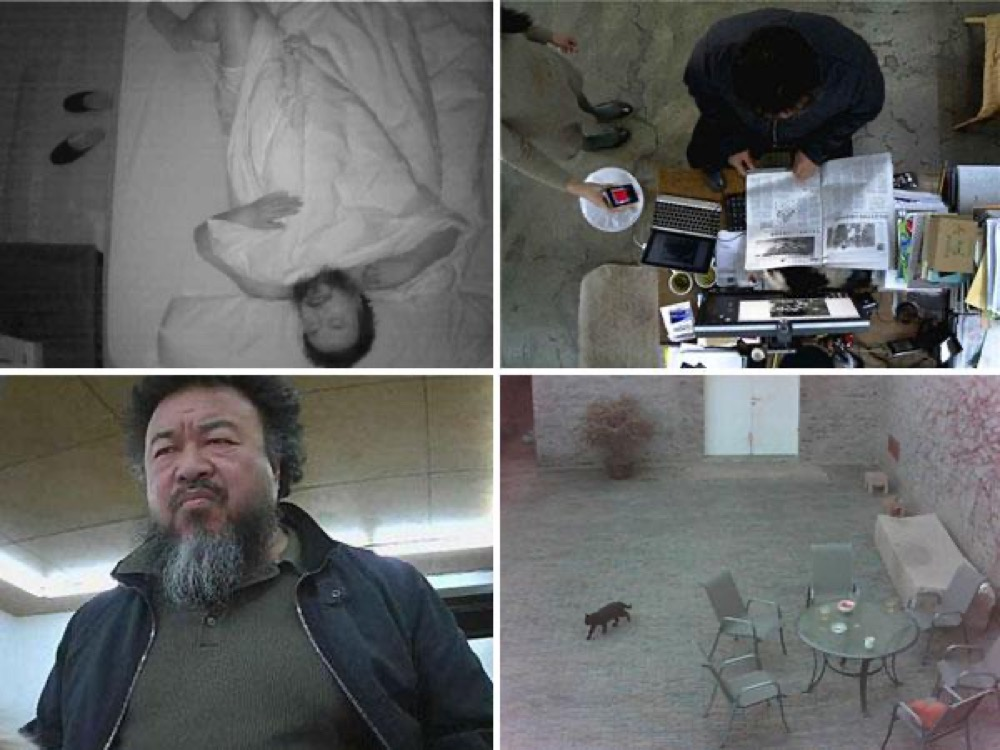
\includegraphics[width=0.75\linewidth,height=0.25\textheight,keepaspectratio]{images/weiweicam.jpg}
  \caption{Weiweicam, by Ai Weiwei, 2012}
  \caption*{Retrieved from \cite{website-forbes-ai-weiwei-cam}}
  \label{fig:weiweicam}
\end{figure}

Another aspect I want to highlight is \textbf{algorithmic bias}. The worlwide release of the documentary Coded Bias on Netflix has helped me find the language to navigate these topics. I am an underrepresented minority, and often it happens to me that supposedly automatic neutral technologies don't understand me. Here is an example of the popular software Zoom, where I spoke out loud "This is a test to show that Zoom transcriptoin does not work with my voice because of my accent", but the words Zoom and voice were transcribed as soon and boys, respectively.

\begin{figure}[ht]
  \centering
  
\includegraphics[width=0.75\linewidth,height=0.25\textheight,keepaspectratio]{images/zoom-introduction.jpg}
  \caption{Screen capture of speech to text on Zoom, introduction}
  \caption*{Screen capture by myself}
  \label{fig:zoom-voice}
\end{figure}

Here is also a further experiment of pronunciation with less common words, in this case, the names of the members of my thesis commitee: Tod Machover, Mitchel Resnick, Zach Lieberman.

\begin{figure}[ht]
  \centering
  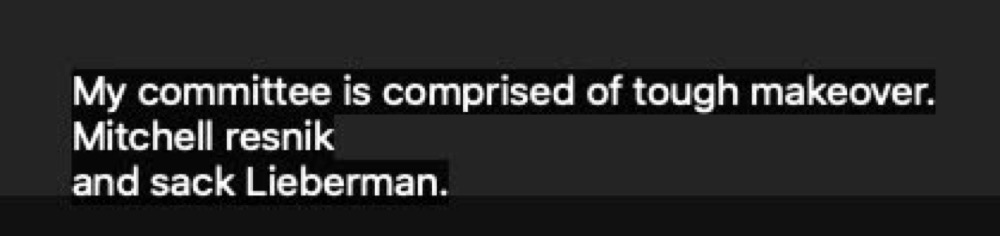
\includegraphics[width=0.75\linewidth,height=0.25\textheight,keepaspectratio]{images/zoom-commitee.jpg}
  \caption{Screen capture of speech to text on Zoom, committee}
  \caption*{Screen capture by myself}
  \label{fig:zoom-committee}
\end{figure}

These examples are not affecting me negatively, but these algorithmic decisions can have devastating effects in equity and discrimination.  Despite \acrshort{ML} algorithms being promoted by corporations and governments as unbiased, most probably these algorithms have never been exposed to Chilean people with my accent.

Because of these errors and my general distrust with these supposedly automatic tools, I routinously turn off voice assistants and text completion in my devices (if you have ever interacted with me over text, I typed every single character :)). I am not comfortable with the widespread commercialization of voice assistants, including Apple's Siri, Amazon's Alexa,  Google's Google Assistant, or Microsoft's Cortana, because I think they are an invasion of privacy.

A year ago, while I was deciding what topic to work on for this thesis, a video \cite{website-talk-technology-and-public-art-rafael-lozano-hemmer} was released of a conversation between artists Rafael Lozano-Hemmer and Dorothy Santos, and on 36m28s Rafael said " Face recognition needs to be banned in all applications except art."

\begin{figure}[ht]
  \centering
  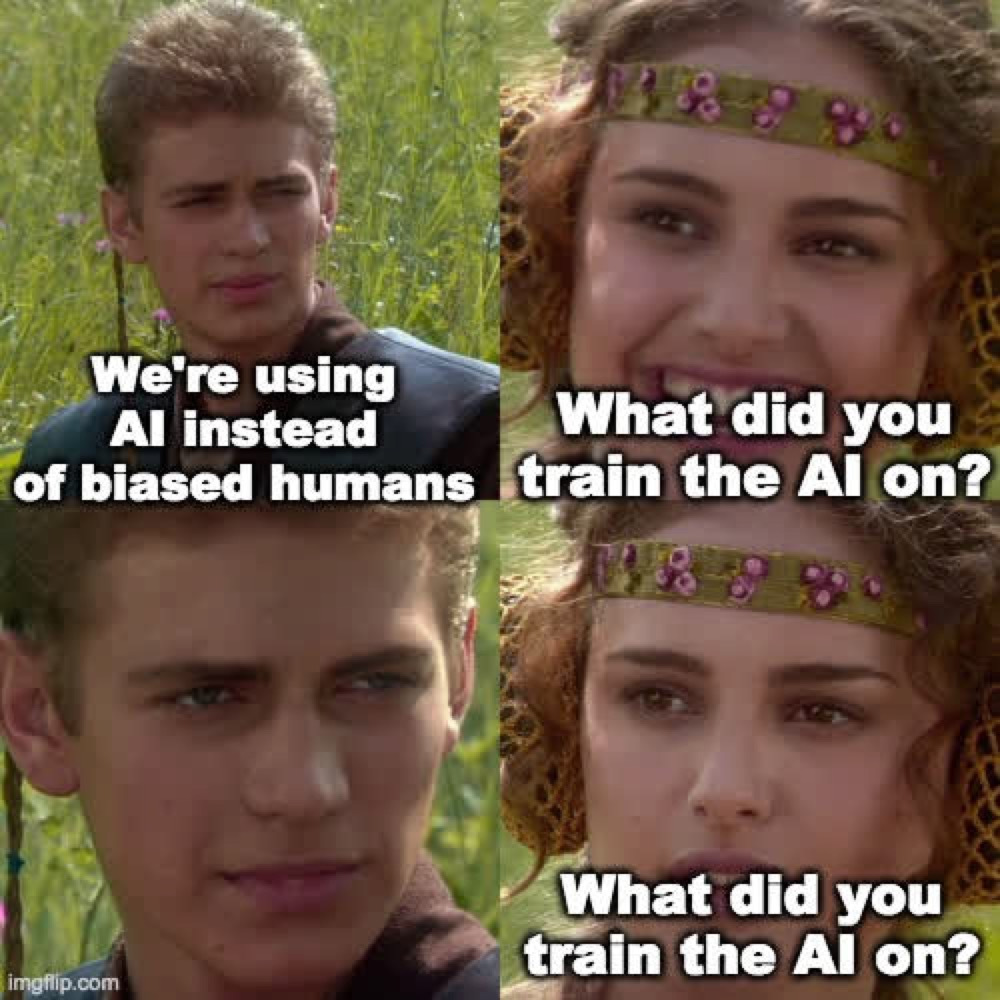
\includegraphics[width=0.75\linewidth,height=0.25\textheight,keepaspectratio]{images/meme-star-wars.jpg}
  \caption{Meme about biased data}
  \caption*{Retrieved from \cite{website-twitter-janellecshane-meme}}
  \label{fig:meme-star-wars}
\end{figure}

This was the perfect spark for starting to work on this project, and make more accesible these computational techniques to beginners, enthusiasts, and educators, to have a more critical and safer use of technology. I highly recommend checking out the important work of the Algorithmic Justice League in these important topics.

We should also not forget that with computational resources becoming cheaper, \acrshort{ML} becomes cheaper, and we can be tempted to use it in applications that don't need in the first place.

\begin{figure}[ht]
  \centering
  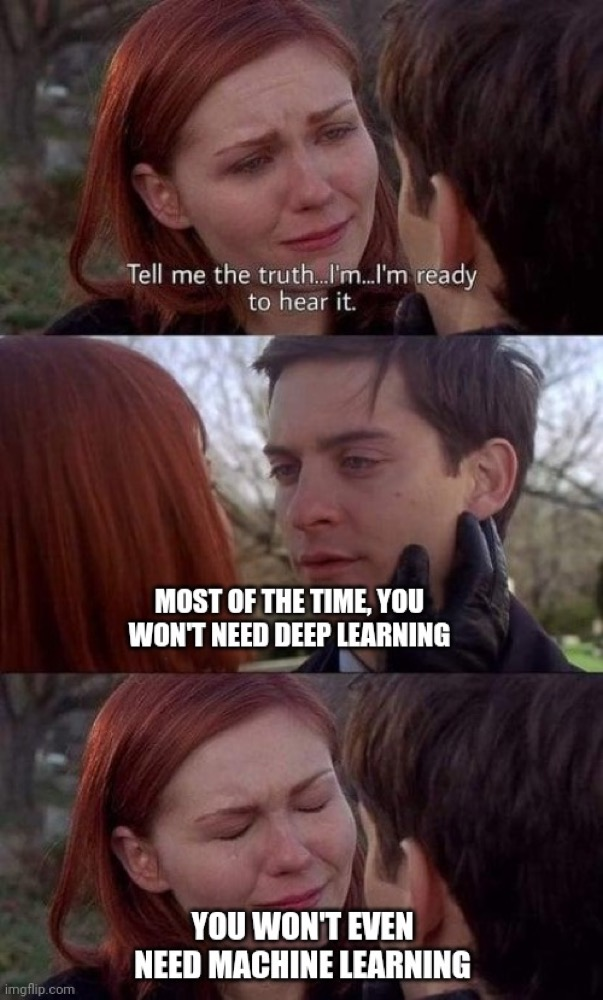
\includegraphics[width=0.75\linewidth,height=0.40\textheight,keepaspectratio]{images/meme-spider-man.jpg}
  \caption{Meme about need of machine learning}
  \caption*{Retrieved from \cite{website-twitter-dynamicwebpaige-meme}}
  \label{fig:meme-spider-man}
\end{figure}

Artists have unprecedented access to new tools for making new tools and instruments, and this thesis intends to be a foundation for a new generation of instruments for manipulating audiovisual material, using \acrshort{ML}. This approach is really exciting because it allows beginners and artists to train their instruments instead of programming them, by inputting data for tuning, instead of having to write lines of code and fixed thresholds for changing their behavior.

My guess is that these errors come from a combination of factors, including my English accent, and the Chilean accent not being widely included on the databases used for training.

The proposal of media arts instruments that can run on little power, rechargeable batteries is a friendly use of resources for experimentation in arts. This is in contrast with the high power use and critique of other emerging fields such as Non Fungible Tokens (NFTs) and cryptoart. The proposal of these scriptable open source instruments allows for users to continuously tweak and modify their instruments, repurpose the hardware, and enable sharing.

\section{Objectives}

With the release of the library Google TensorFlow Lite Micro, the TinyML Foundation, new avenues have been opened for creative expression using \acrshort{ML} in microcontrollers.

TensorFlow is a library by Google for \acrshort{ML}. They have released different flavors for different devices, including TensorFlow.js for working with KavaScript and in the browser, and TensorFlow Lite for devices with less memory, like mobile devices. The newer TensorFlow Lite Micro is even lighter and intended for working on microcontrollers, and that is the flavor I am using in this thesis.

in a paragraph here that combines the points you make in the first paragraphs -> the main contributions of YOUR thesis... which it seems is basically just addressing a bunch of the context section? Blakeley Payne's thesis does a good job of outlining contributions. It's also good to do here to understand where you are going

Homebrew examples, teach people how to build their own databases, and how to circumvent corporations view.

TODO: Terms and conditions comic book. If people were to read terms and conditions, it would take them X years

You can train an instrument to only detect your voice, your accent, your living conditions.

TODO: Raspberry Pi example, it’s cheap but it needs a lot of extra hardware to be used

Navigating legal documents can be hard. In 2010, GameStation added a soul clause to their terms of conditions as an April Fool's prank, making them legal owners of thousands of customers' souls \cite{website-huffpost-gamestation-soul-clause}. And back in 2007, it was estimated that people would need around 250 hours every year to actually read the privacy policies shown to them \cite{article-cost-of-reading-privacy-policies}.

\section{Some dreams}

Infrastructure and cooperation are key, I love how I can bike on roads and hike on paths, and I hope this work can be adopted by fellow artists and educators to create new instruments for arts, and for making new laws that curb algorithmic bias.

TODO: insert picture of surveillance camera near my home, in the middle of nature.

I hope this work can be taken to the next step, by building a new generation of private and smart devices, like one of my first dreams, a drum machine I can talk to, and ask for different rhythms mid performance, or using my body gestures to write poems.

\section{Thesis outline}

This thesis has cover the following chapters:

\begin{enumerate}
  \item Chapter 1, Introduction: the context and summary of this thesis.
  \item Chapter 2, Tiny trainable instruments: description of the design strategies for the software and hardware, description of the support team working on this thesis.
  \item Chapter 3, Early experiments: my earlier work that led to this thesis, in the topics of media arts education, microcontrollers, and \acrshort{ML}, among others.
  \item Chapter 4, Background and inspiration: work by other people which has informed my work.
  \item Chapter 5, Project evaluation: user feedback, field notes.
  \item Chapter 6, Conclusions and future work: next iterations of the instruments, and their proposed use for educators and artists.
  \end{enumerate}
